\section{Inspiral Trigger Generation}
\label{s:trigger}

We search for inspiral signals in the LIGO data with a matched
filtering\cite{wz} algorithm implemented in the \emph{findchirp}
package\cite{findchirp} of the LIGO/LSC Algorithm library\cite{lal}. The LIGO
data is recorded at a sampling rate of $16384$ Hz.  The highest frequency of
gravitation radiation that we are searching for is approximately $2200$ Hz and
so we resample the data to $4096$ Hz for the matched filtering.  An 8th order
Butterworth filter was applied to the interferometer data which attenuated the
signal by $10\%$ at $100$ Hz. This prevented numerical corruption of the power
spectral estimate due to large power in the LIGO noise curve at low
frequencies. Initial analysis of the data from the L1 interferometer
discovered that a large non-stationary noise source at around $60$---$70$~Hz
was producing an excessive number of inspiral triggers. A low frequency cutoff
was applied in the frequency domain by setting the data to zero at frequencies
below $100$ Hz.  The shape of the noise power spectra was such that this did
not produce a significant loss in inspiral range. 

Data is analyzed in $2048$~sec \emph{analysis chunks} consisting of fifteen
$256$~sec \emph{analysis segments} which are overlapped by $128$~sec. A median
power spectrum is computed for each of these analysis segments; for each
frequency bin, the median value of the $15$ power spectra is used to
calculate the average power spectrum used in the matched filter.  A
\emph{template parameter bank} is used to generate second order post-Newtonian
templates in the frequency domain using the stationary phase approximation to
the inspiral signal. For a given template
and analysis segment we construct the signal-to-noise ratio, $\rho$,  and
search for times when this exceeds a threshold,  $\rho > \rho^\ast$. If this
happens, we construct a template based veto, the $\chi^2$
veto\cite{brucechisq}. Small values of $\chi^2$ indicate that the
signal-to-noise was accumulated in a manner consistent with an inspiral
signal. If the value of the $\chi^2$ veto is below a threshold, $\chi^2 <
{\chi^2}^\ast$, then an inspiral trigger is recorded at the maximum value of
$\rho$. For a given template multiple triggers can be recorded in a segment.
The triggers are clustered so that distinct triggers are separated by at least
the length of the template.  Each analysis segment is filtered through all the
templates. It is possible for multiple templates to trigger at same time.
Details of the template banks passed to the trigger generation code are
described in the next section. 

\section{Data Analysis Pipeline}
\label{s:pipeline}

The interferometer operators, in consultation with scientific monitors present
at the observatory during data taking, flag times when the interferometers are
in stable operation and the data is suitable for analysis.  Further studies of
the raw data yield a series of \emph{data quality cuts} that are used to
exclude anomalous data from the inspiral analysis\cite{gwdawveto}. We have
excluded times when \emph{(i)} servo controls in the L1 interferometer were
set incorrectly, \emph{(ii)} calibration information is unavailable for the
analysis, \emph{(iii)} there are photodiode saturations, \emph{(iv)} data has
invalid time stamp information and \emph{(v)} the noise in the H1
interferometer is significantly larger than average. In general, the
interferometer is considered to be malfunctioning during these times with the
exception of \emph{(i)} and \emph{(ii)} which are due to operator error. In
the case of \emph{(v)}, we ensure that the increased noise is not due to the
presence of an inspiral signal in the data by only excluding times when the
noise is excessive for more than $180$~sec, which is significantly longer that
our longest inspiral signal of $3.7$~sec.

As can be seen from figure~\ref{f:s2noisecurve} and the average sensitivity
during S2, the range of the L1 detector is approximately twice that of the H1
detector, which is larger than that of the H2 detectors. At all times during
the run L1 is more sensitive than H1 and H1 is more sensitive than H2. We use
this and the fact that we demand that a trigger be present in multiple
interferometers to construct a \emph{triggered search pipeline}. This allows
us to save a significant amount of computational effort during the search,
without reducing the detection efficiency. Here we illustrate the method of
the triggered search for two interferometers. Further details of the triggered
search pipeline for multiple interferometers can be found in
reference~\cite{abbott2004a}.

For each analysis chunk a template bank is generated for the L1 detector for
binary neutron stars with component masses between $1.0$ and $3.0 M_\odot$, as
described in \cite{owensathya}.  The \emph{minimal match} of the bank is
chosen to be $0.97$. A random inspiral signal lying in the space of the bank
would lose no more than $3\%$ of the signal-to-noise ratio due to mismatch
between the signal and the nearest template. We filter each L1 analysis chunk
through the corresponding bank to generate inspiral triggers. We then select
each template from the L1 bank that produced one or more inspiral triggers to
construct a \emph{triggered bank.} The triggered bank, which is a subset of
the original template bank, is used to filter the data from the less sensitive
interferometer (e.g. the H1 detector) to produce a second list of inspiral
triggers. We demand coincidence between triggers from the different
interferometers, as described below, to produce the list of \emph{coincident
triggers.} We apply instrumental vetoes to this list of coincident triggers to
exclude triggers that are due to known instrumental or environmental artifacts
in the data, as described in \cite{gwdawveto}. Any surviving triggers are
considered to be the list of candidate inspiral triggers from the analysis.

To perform the triggered search pipeline on the full data set, we constructed
a directed acyclic graph (DAG) that described the work flow.  The DAG is
executed using the Condor high throughput computing system\cite{condor} on the
UWM and Caltech bewoulf clusters.

\section{Trigger Coincidence}
\label{s:coincidence}

For a trigger to be considered coincident in two interferometers, we demand
that it is observed in both interferometers within a temporal coincidence
window $\delta t$. Monte Carlo analysis with simulated signals suggests that we
cannot measure the time of the trigger to an accuracy of less than $1$~ms, so
we demand $\delta t = 1$~ms if the interferometers are located at the same
observatory. If the detectors are not co-located, we allow for the $10$~ms
light travel time between the LIGO observatories by demanding $\delta t =
11$~ms. We also demand that the waveform of the triggers are consistent by
requiring that the two mass parameters, $m_1$ and $m_2$, of the binary are
identical.

\begin{figure}
  \vspace{5pt}
  \begin{flushright}
    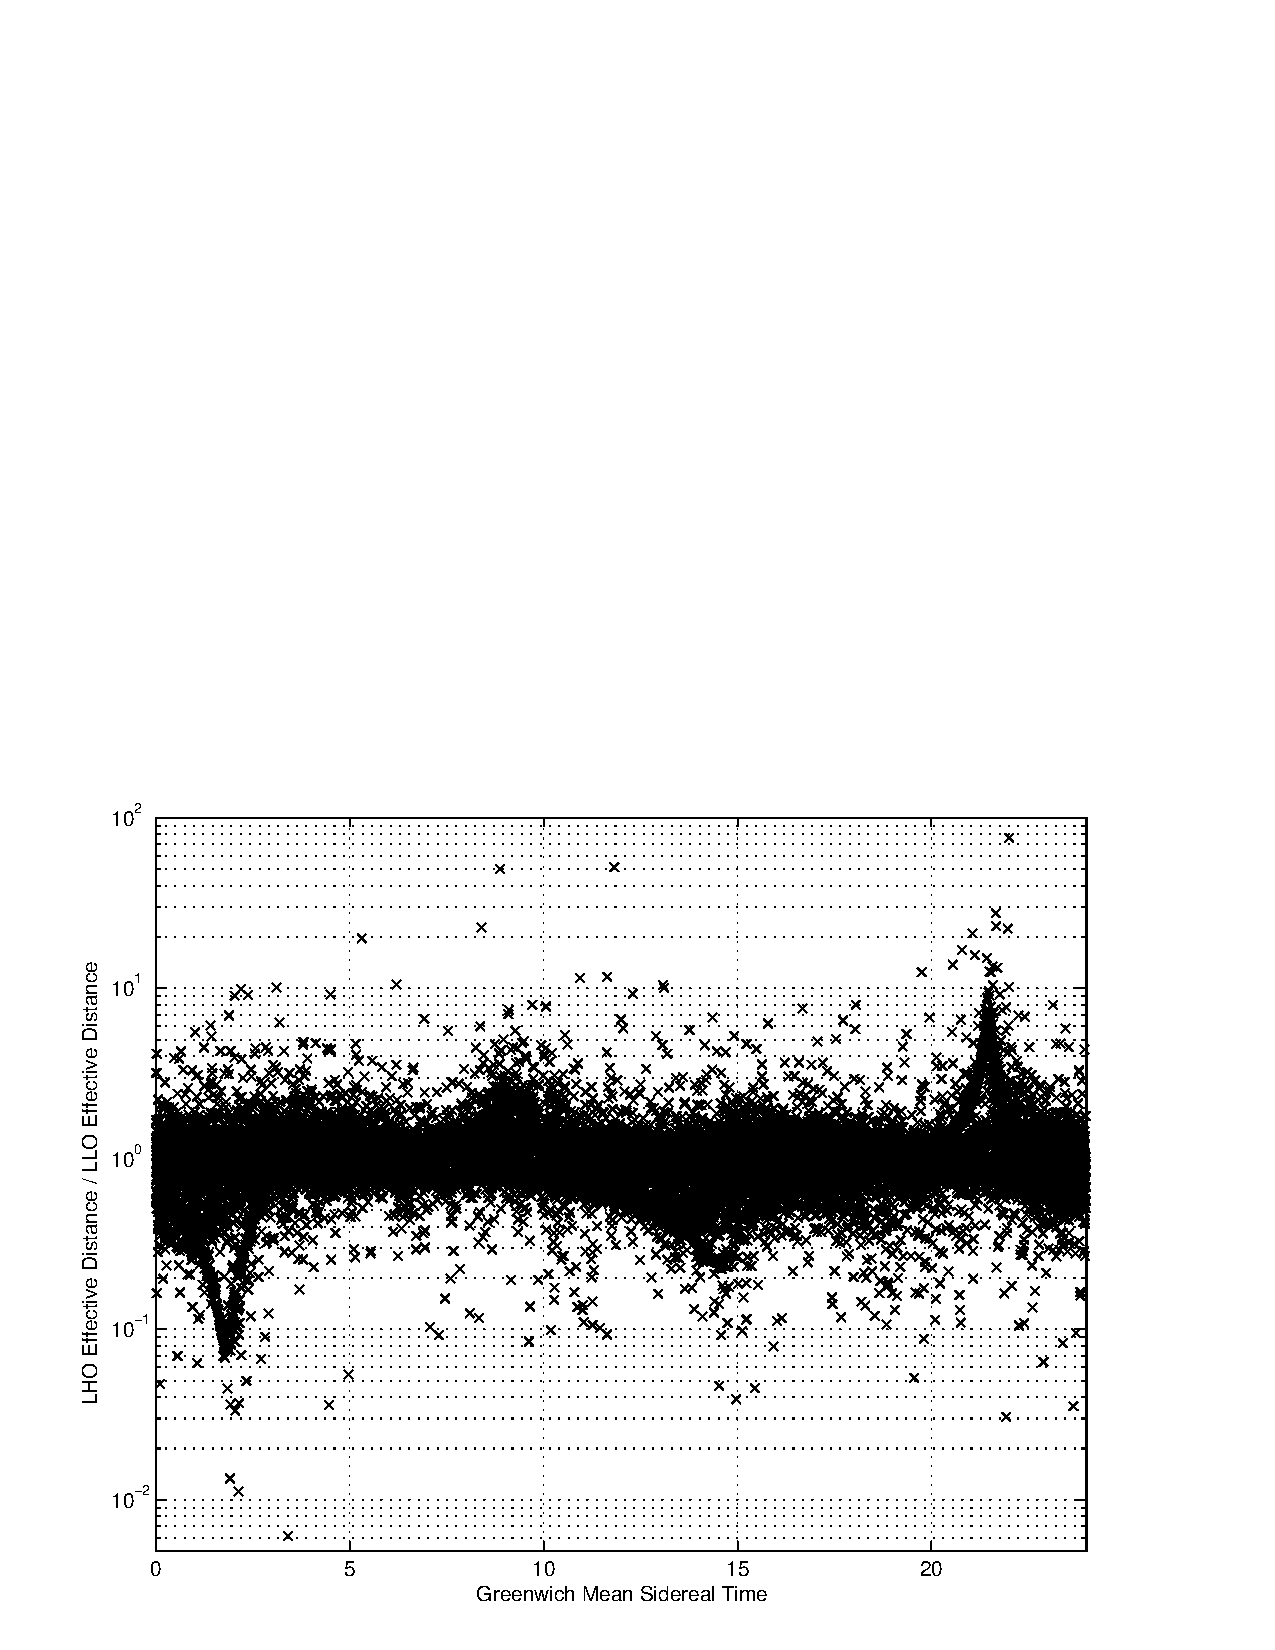
\includegraphics[width=\textwidth]{gmst_dist_ratio}    
  \end{flushright}
  \caption{%
  The ratio of the known effective distance of an injected signal in the
  Hanford Observatory (LHO) to the known effective distance of an injected
  signal in the Livingston Observatory (LLO) as a function of Greenwich Mean
  Sidereal Time. The slight misalignment of the interferometers at the two
  different observatories due to the curvature of the earth causes the antenna
  pattern of the detectors to differ. As a result the distance at which a
  binary system appears is different in each detector, even in the absence of
  noise.  The ratio of effective distances can be significant, so this
  precludes the use of an amplitude cut when testing for inspiral trigger
  coincidence between different observatories.
  }
\label{f:gmst_dist_ratio}
\end{figure}
We now consider an amplitude cut on the signals. The Livingston and Hanford
detectors are not co-aligned. There is a slight misalignment of the detectors
due to the curvature of the earth and so the antenna patterns of the detectors
differ. This causes the measured amplitude of a gravitational wave to differ
between the sites. In the extreme case, it is possible for a binary to be
completely undetectable by the L1 detector, but still detectable by the H1 and
H2 detectors. For a given inspiral trigger, we measure the \emph{effective
distance} of the binary system. This is the distance at which an optimally
oriented binary would produce the observed signal-to-noise ratio.
Figure~\ref{f:gmst_dist_ratio} shows the ratio of effective distances between
the two LIGO observatories for the population of binary neutron stars
considered in the S2 analysis. The significant variation of the effective
distance precludes using a naive test for amplitude coincidence. It is
possible to obtain information about sky position from time delay between
sites to construct a more complicated amplitude cut, but this has not be used
in the S2 analysis.

In the case of triggers from the H1 and H2 interferometers that are coincident
in time and mass, we apply an amplitude cut that tests that the effective
distance of the triggers is coincident given the relative sensitivity of the
detectors, while allowing for error in this measurement which is determined by
Monte Carlo simulations.  When testing for triple coincident triggers we 
accept triggers that are coincident in the L1 and H1 detectors that are
\emph{not} present in the H2 detector \emph{if} the effective distance of the
trigger is further than the maximum distance of H2 at signal-to-noise ratio
$6$ at the time of the candidate trigger.

As in the S1 analysis, the list of surviving candidate triggers is followed up
by examining the raw gravitational wave data, axillary interferometer channels
and physical environment monitoring channels to determine if the triggers are
truly of astrophysical origin.

\section{Background Estimation}
\label{s:background}

Since we restrict the S2 analysis to coincident data and require that at least
two of the interferometers must be located at different observatories, we may
measure a background rate for our analysis. After generating triggers for each
interferometer, we slide the triggers from one observatory relative to the
other observatory and look for coincidences between the shifted and unshifted
triggers. The minimum slide length is chosen to be greater than the length of
the longest filter ($20$~sec) so any coincident triggers detected must be due to background and
not astrophysical events. By examining the distribution of background events
in the $(\rho_\mathrm{H},\rho_\mathrm{L})$ plane we can attempt to determine
contours of constant false alarm rate in order to construct a combined
effective signal-to-noise ratio for a coincident trigger\cite{abbott2004a}.

\section{Detection Efficiency}
\label{s:eff}

In absence of detection, we will construct an upper limit on event rate.  To
do this, need to measure the detection efficiency of the analysis pipeline to
our population. A Monte Carlo method is used to measure this efficiency. We
simulate a population of binary neutron stars and \emph{inject} signals from
that population into the data from all three LIGO interferometers. The
injection is performed in software by generating an inspiral waveform and
adding it to interferometer data immediately after the raw data is read from
disk. We inject the actual waveform that would be detected in a given
interferometer accounting for both the masses, orientation, polarization, sky
position and distance of the binary, the antenna pattern and calibration of
the interferometer into which this signal is injected.  The effectiveness of
software injections for measuring the response of the instrument to an
inspiral signal is validated against \emph{hardware injections}\cite{hw} where
an inspiral signal is added to the interferometer control servo during
operation to produce the same output signal as a real gravitational wave.  The
data with injections is run through the full analysis pipeline to produce a
list of inspiral triggers. The detection efficiency of the pipeline,
$\epsilon$, is the ratio of the number of detected signals to the number of
injected signals.
